\section{Zähler} % (fold)
\label{sec:Zähler}
\begin{frame}
    \frametitle{Zähler}
    \framesubtitle{}
     \begin{figure}[H]
     \begin{center}
             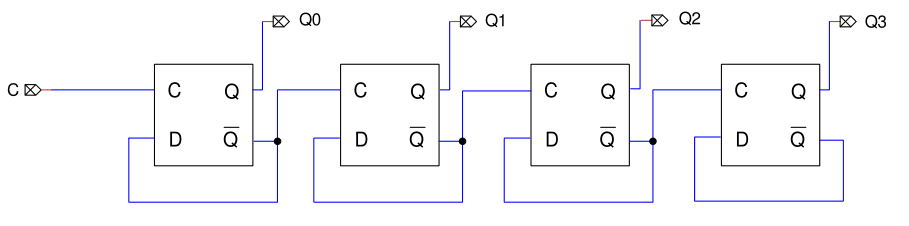
\includegraphics[scale=0.3]{./img/schaltung/zahler.png}
     \end{center}
     \end{figure}
\end{frame}
\begin{frame}
    \frametitle{Entwicklung}
    \framesubtitle{}
    \begin{columns}[c]
        \column{0.5\textwidth}
         \begin{block}{Funktionsweise}
            \begin{itemize}
                \item D-Latch flipt aktuelles Bit 
                \item falls Q gesetzt wird $\bar{Q}$ und somit der nächste D-Latch
                gesetzt
                \item Zahl muss 'rückwärts' gelesen werden
            \end{itemize}
         \end{block}
        \column{0.5\textwidth}
             \begin{center}
                \boxed{
                    \begin{tabular}{c}
                        0000 \\
                        1000 \\
                        0100 \\
                        1100 \\
                        0010 \\
                        1010 \\
                        1110 \\
                        0001 \\
                        1001 \\
                        0101 \\
                        1101 \\
                        0011 \\
                        1011 \\
                        0111 \\
                        1111 \\
                    \end{tabular}
                }
             \end{center}
    \end{columns}
\end{frame}
% section Zähler (end)
